% !TEX root = Heuberger_Petracci_reflID_735.tex


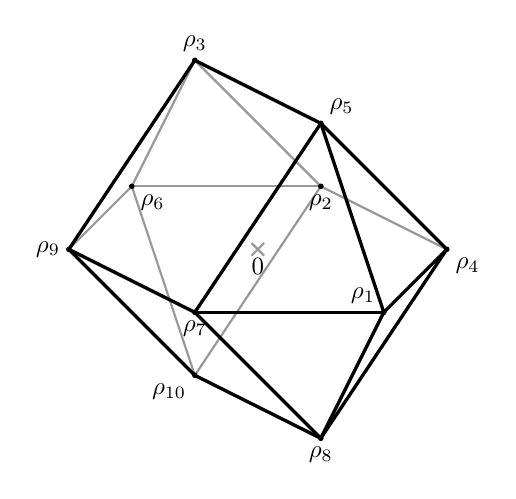
\begin{tikzpicture}[scale=0.8,every node/.style={scale=0.9}]
%background edges
\draw[gray!80, thick] (1,1) -- (-2,1);
\draw[gray!80, thick] (1,1) -- (-1,3);

\draw[gray!80, thick] (1,1) -- (3,0);
\draw[gray!80, thick] (-1,3) -- (-2,1);
\draw[gray!80, thick] (-3,0) -- (-2,1);
\draw[gray!80, thick] (1,1) -- (-1,-2);
\draw[gray!80, thick] (-1,-2) -- (-2,1);


%foreground edges
\draw[black, very thick] (-3,0) -- (-1,3);
\draw[black, very thick] (-3,0) -- (-1,-1);
\draw[black, very thick] (-1,-1) -- (1,2);
\draw[black, very thick] (1,2) -- (3,0);
\draw[black, very thick] (1,2) -- (2,-1);
\draw[black, very thick] (-1,-1) -- (2,-1);
\draw[black, very thick] (2,-1) -- (3,0);
\draw[black, very thick] (1,2) -- (-1,3);
\draw[black, very thick] (3,0) -- (1,-3);
\draw[black, very thick] (2,-1) -- (1,-3);
\draw[black, very thick] (-1,-2) -- (1,-3);
\draw[black, very thick] (-1,-2) -- (-3,0);
\draw[black, very thick] (-1,-1) -- (1,-3);

%origin 
\draw[gray!80, thick] (0.1,0.1) -- (-0.1,-0.1);
\draw[gray!80, thick] (-0.1,0.1) -- (0.1,-0.1);


%nodes
\filldraw[gray] (0,0) circle (0pt) node[anchor=north] {\textcolor{black}{$0$}};
\filldraw[black] (2,-1) circle (1pt) node[anchor=south east] {$\rho_1$};
\filldraw[black] (3,0) circle (1pt) node[anchor=north west] {$\rho_4$};
\filldraw[black] (1,1) circle (1pt) node[anchor=north] {$\rho_2$};
\filldraw[black] (-2,1) circle (1pt) node[anchor=north west] {$\rho_6$};
\filldraw[black] (-3,0) circle (1pt) node[anchor=east] {$\rho_9$};
\filldraw[black] (1,-3) circle (1pt) node[anchor=north] {$\rho_8$};
\filldraw[black] (-1,-2) circle (1pt) node[anchor=north east] {$\rho_{10}$};
\filldraw[black] (1,2) circle (1pt) node[anchor=south west] {$\rho_5$};
\filldraw[black] (-1,3) circle (1pt) node[anchor=south] {$\rho_3$};
\filldraw[black] (-1,-1) circle (1pt) node[anchor=north ] {$\rho_7$};



%\filldraw[black] (5,-3) circle (1pt) node[anchor=north west] {$(1,1,-1)$};
%\filldraw[gray] (2,-2) circle (1pt) node[label={[xshift=-0.9cm, yshift=-0.3cm]\textcolor{black}{$(0,1,-1)$}}]{};
%\filldraw[gray] (-6,-7) circle (1pt) node[label={[xshift=1.3cm, yshift=-0.3cm]\textcolor{black}{$(-1,-2,-2)$}}]{};
%\filldraw[black] (-2,-10) circle (1pt) node[anchor=north] {$(1,-3,-2)$};
%
%\filldraw[gray] (0,-3) circle (1pt) node[anchor=south east]{};
\end{tikzpicture}



